\documentclass{sig-alternate}
\usepackage[latin1]{inputenc}
\usepackage{url}
\usepackage{listings}
\usepackage{subfigure}
\newfont{\mycrnotice}{ptmr8t at 7pt}
\newfont{\myconfname}{ptmri8t at 7pt}
\let\crnotice\mycrnotice%
\let\confname\myconfname%

\permission{Permission to make digital or hard copies of part or all of this work for personal or classroom use is granted without fee provided that copies are not made or distributed for profit or commercial advantage, and that copies bear this notice and the full citation on the first page. Copyrights for third-party components of this work must be honored. For all other uses, contact the owner/author(s). Copyright is held by the author/owner(s).}
\conferenceinfo{GECCO'14,}{July 12--16, 2014, Vancouver, BC, Canada.}
\copyrightetc{ACM \the\acmcopyr}
\crdata{978-1-4503-1964-5/14/07. \\
Include the http://DOI string/url which is specific for your submission and included in the ACM rightsreview confirmation email upon completing your ACM form}

\clubpenalty=10000
\widowpenalty = 10000
\begin{document}
%
% --- Author Metadata here ---
\conferenceinfo{GECCO'14} {Vancouver, Canada}

\title{A Methodology for Designing Emergent Literary Backstories on Non-player Characters using Genetic Algorithms}
\subtitle{}
\numberofauthors{2}
\author{
\alignauthor
R. H. Garc{\'i}a-Ortega\\
       \affaddr{Fundaci{\'o}n I+D del Software Libre}\\
       \email{rhgarcia@fidesol.org}
\alignauthor
P. Garc{\'i}a-S{\'anchez}, A. M. Mora and J.J. Merelo\thanks{This work has been developed thanks to the funds provided by the ANYSELF project (TIN2011-28627-C04-02). }\\
\affaddr{GeNeura, ETSIIT + CITIC}\\
\affaddr{University of Granada}\\
\email{pgarcia,amorag,jmerelo@geneura.ugr.es}
}

\maketitle
\begin{abstract}
%Stories are not only painfully weaved by crafty writers in the
%solitude of their studios; they also have to be produced massively for
%non-player characters in the video game industry or tailored to
%particular tastes in personalized stories. However, the creation of
The creation of fictional stories is a very complex task that usually implies a
creative process where the author has to combine characters, 
conflicts and backstories to create an engaging narrative.
This work presents a general methodology that uses individual based models to generate cohesive and coherent
backstories where desired {\em archetypes} (universally accepted literary symbols) emerge and their life stories are a by-product of the simulation.
This methodology includes the modeling and parameterization of the agents, the environment where they will live and the desired literary setting. The use of a genetic algorithm (GA) is proposed to establish the parameter configuration that will lead to backstories that best fit the setting. Information extracted from a simulation can then be used to create the backstories.
To demonstrate the adequacy of the methodology, we perform an implementation using a specific multi-agent system and evaluate the results.
%, which show that {\em archetypes} can emerge and that the optimal number of profiles (or set of parameters assigned to the agent) depends on the target setting. % and the results are... - JJ

\end{abstract}

% A category with the (minimum) three required fields
\category{H.4}{Information Systems Applications}{Miscellaneous}
%A category including the fourth, optional field follows...
%\category{G.1.6}{Mathematics of Computing}{NUMERICAL ANALYSIS}[Optimization]

\keywords{Genetic Algorithms, literature, content generation}

\section{Introduction}
Non-Player Characters (NPCs) in video games are a type of characters % repite character
that live in the game world to provide a more inmersive
experience and, in some cases, present a challenge to the human player.
%Modern  Role Playing Games (RPGs), such as The
%Witcher\texttrademark~or Skyrim\texttrademark~ include hundreds of NPCs. The effort to create a good interactive fiction script is directly proportional to the number of these characters. Thus, this kind of agents usually present limited behaviors, such as wandering in the villages, selling groceries or guarding the cities. These characters are frequently programmed to interact with the human player, following a guided sequence of activities just with this purpose, so normally they do not interact among themselves.
Games can include hundreds or even more NPCs, and their collective interactions  improve the gaming experience and lead to a richer and more inmersive world. But inmersion is not guaranteed and can only be achieved if the characters backstory is coherent and also diverse. % he a�adido esto porque no hab�a "Facts" a los que te refieres en la frase siguiente - JJ
which motivated us to develop a methodology to generate backstories by modeling the language, agents and a literary setting based in the concept of {\em archetypes}, behaviors and patterns universally accepted and
present in the collective imaginary. This methodology is able to 
create massive backstories % �fondos de pantalla? usad un lenguaje preciso - JJ
 for secondary characters, in order to provide a context for the writer and the
player to perceive a virtual world as coherent, detailed and
enriched.

To validate our methodology we have released a multi-agent system called
MADE (Massive Artificial Drama Engine) that models a self-organized
virtual world where every element influences each other, following
cause-effect behaviors in a coherent manner.
%This system must be
%a suitable environment for the plot of a specific literary work, also being
%interesting for the player/spectator.
We have followed the ideas of the work 
\cite{epstein1996growing}, 
the first widely known multi-agent generative social model. As a step of the methodology, a self-organizing system is defined following the methodology introduced in
\cite{gershenson2005general}: a virtual world, agents who are born, grow, 
interact, reproduce and dead; resources (food), mediators, and
relations of rivalry (friction) and cooperation (synergy). In other step of our methodology, the actions of the agents are parametrized according the work 
\cite{nairat2011character}, based on the use of GAs in order to
obtain a plot (solution) where two characters interact in a creative way.
The narrative is addressed by our methodology as the final step,
giving freedom to creators. This issue has been studied in the systems presented on the review \cite{ReviewArinbjarnar09}.

In this paper we show that GAs, together with a proper design of
literary patterns and archetypes, can be used to find the parameters that promote the
generation of drama plots and sub-plots in a multi agent based
environment.
%The rest of the work is structured as follows: after the state of the art, the proposed methodology is presented in Section \ref{sec:methodology}. Then, some experiments, showing possible applications of this methodology (including the GA application) are presented (Section \ref{sec:applying}). Finally, conclusions and future work are discussed.
%Previous works define the plot as as something that emerges from the behavior of the agents that follow a set of rules. In the proposed methodology, the agents' behaviour is produced by their personality and the environment. That is, the agents do not follow a plot, but they generate the plot itself.
%
%Furthermore,  previous works generate plots in worlds with a limited number of characters. This restriction does not exist in our methodology, where the number of characters to create is unlimited: They are created massively and their goal is to relate in a complex system and generate backgrounds that fit the setting of a plot, not the plot itself.
%The proposed methodology is innovative since the goal has not been addressed before. Previous researches are focused on the plot, the interaction, and the narrative, but our proposal is focused on backgrounds (not in plot), where different archetypes emerge involving a starting point for future plots and subplots.


%According to the taxonomy described by Togelius et al. \cite{Togelius2011}, the present methodology can be classified as a \textit{procedural content generator} (\textit{PGC})
%mainly related to \textit{optional content}, with \textit{stochastic generation}
%and modeled as a \textit{generate-and-test} algorithm (search based), that
%performs the optimizations of the process during the game development
%(\textit{offline}). % este p�rrafo deber�a ir a la intro JJ PPSN



%
%%%%%%%%%%%%%%%%%%%%%%%%%%%%%%%   METHODOLOGY   %%%%%%%%%%%%%%%%%%%%%%%%%%%%%%%
%

\section{Methodology and Application}
\label{sec:methodology}

%The mood, or the atmosphere, of the literary setting is one element in the narrative structure of a piece of literature. It is established in order to affect the reader emotionally and psychologically and provide a feeling for the narrative.


%The present methodology defines different steps that will lead the user from the initial question ``\textit{How could I obtain secondary characters for my setting, with coherent backstories consistent with its mood?}'' to a system that can automatically generate a setting massively populated with characters and backstories, where different desired behaviors or archetypes emerge from their interactions.


%These archetypes, conceptually modeled, would be designed and instantiated as regular expressions over a language used to describe the backstories along with the social relationships between them. Those instantiations will be used by the GA to obtain the fitness of each solution. The process is iterative and presented as a waterfall model, where each step influences the following one.
%The methodology includes the following steps:  modeling - the
%language, the literary setting, the agent -, definition of the GA
%characteristics, instantiation, execution, which will be exposed in
%the following subsections, and finally interpretation. 



%\subsection{Modeling} 
In our approach, the mood of the setting will be modelled as a group of abstract archetypes and different conditions over them.
Initially, each agent has to be modelled as a Finite State Machine (FSM) whose transitions generate symbols in a language that includes dates, actions, direct and indirect objects.
% based on the following one, expressed in Backus-Naur Formalism (BNF):
%
%\begin{verbatim}
%<backstory> ::= <action_line> [<backstory>]
%<action_line> := <date> <action>;
%<action> = <action_id> [<direct_object>]
%           [to <indirect_object>]
%\end{verbatim}
%Starting from this partial grammar, the user has to define the expressions:
%\begin{itemize}
%\item \textbf{<date>}: Should be expressed in a way that is meaningful
%  to the type of background that we are looking for. For example, if we are talking about persons, it could be the age of the agent expressed in days.
%
%\item \textbf{<action\_id>}: Different actions can be taken into
%  account, and will depend on the kind of archetypes we will look
%  for. For example, if we are trying to find archetypes about love
%  like the classical Romeo and Juliet one, where two characters are in
%  love but belongs to families in war and finally ends up with their
%  death, we could include actions and relations like ``loves'',
%  ``hates'', ``is son of'', ``is daughter of'', ``is parent of'',
%  ``die'', etc. 
%
%Obviously, the smaller the group of possible actions is, the easier would be to find out the archetypes. In order to minimize the number of available actions and maximize the number of archetypes they allow we propose generic actions instead of specific ones.
%
%\item \textbf{<direct\_object>}: The possible values of the direct objects depend on the nature of the actions.
%
%\item \textbf{<indirect\_object>}: Should define the unique id of an agent or a group of agents.
%
%\end{itemize}
%The backstory generated by each agent using the language modelled this way will be automatic and human readable. Eventually, the backstories will evoke archetypes and behaviors.
%As we will see in the next sections, we will try to promote the emergence of specific archetypes in order to retrieve the best backstories for our setting.
%In a top-down approach (the opposite to the one proposed in the current methodology), if the creative needs a second character or an extra for a story, he or she creates it out of the blue, with the background that better fits with his/her needs. This approach, valid for a small amount of characters and poor requisites of coherence between them, becomes more and more complex when we add more characters to the environment, because each addition implies new relations in their social network.
%
%
%Otherwise, the bottom-up approach promotes the agent as one of the pillars of the system because it offers the coherence of the backstory regarding to the timeline (for example, an agent cannot die before he or she is born). Some actions need to be sequential and to the relations (many actions involve two different agents). An agent is just a simple tool to generate a background, a character. In an environment where many characters can ``live'', make decisions taking into account the other characters and affecting them, the generated background becomes complex, many links have been created and no creative process has taken part on it (the creative process is present in the definition and modeling of the agent itself).
%
%Given this premise, a multi-agent system seems promising for generating this kind of complex relations and backstories.
%
%An agent can be seen as a Finite State Machine (FSM), so the multi-agent system relies in the sequential executions of time portions. Every execution implies a review of the current state and (maybe) one or more actions done, depending on local and external properties.\\
%
%Given a set of states, properties and actions modeled, the logic of the main process should be:
%
%\begin{enumerate}
%\item Collect internal and external information.
%\item Depending on the state and the information collected, select the possible actions and probabilities to perform them.
%\item Use random numbers to decide the action to perform.
%\item Generate an action line using the language selected in the previous stage.
%\item Select the new state.
%\end{enumerate}
%
%
%The agent should contemplate different states depending on the type of information we are interested in (``alive'', ``dead'', ``pregnant'', etc) and should also have local properties that define the possibility to make certain decisions.
%It is important to remark that an agent is a simplification of the character (in the way that it will perform only the actions we are interested in) and that the agent is inspired in conceptual behaviors, so some actions and transitions are mandatory and depend on the personality and internal states.\\
%Agents live in an {\em environment}, understood as the virtual spatio-temporal frame where the agents play their lives. This environment is also responsible for:
%\begin{itemize}
%\item execute the main process of each agent (corresponding to a portion of time). Each iteration the agents should be chosen randomly or based on classical role-playing games features like ``initiative''.
%\item provide a set of functions to interact with other characters and the environment itself.
%\end{itemize}
%The key in the use of agents to create background for characters relies in the following fact: Some actions are performed statically depending on the inputs and the current state but other (the majority) also depends on agent's local features and probabilities. Even if all the agents share these values, it is difficult to predict the result when the system is so complex. A minimal change in one probability to make one decision can imply completely different scenes.
%For this reason, some actions should be statically defined and others have to depend on initialization properties. We define two kind of properties:
%
%
%\begin{itemize}
%\item \textbf{Base properties}: Those that are intrinsically defined by the nature of the conceptual agent. For example, if we are modeling a simplification of a person, the average life expectancy could take values from 70 to 85 years. An agent that lives 100 years would be unusual, and an agent that lives 200 years should not be possible.
%\item \textbf{Searchable properties}: Those used to increment or decrement the base values in the established limits or those that are used directly as probabilities to make decisions.
%\end{itemize}
%
%Due to the complexity of the system and the introduction of probabilities, even if all the agents have the same features and probabilities, the sequence of the actions for every agent becomes unpredictable.
%For example, if we have our agent modeled and we choose random values for the configuration, roughly, the characters' backstories will be ``normal'', showing more or less the stereotyped behaviors (that make the character a group representative rather than an individual), but maybe, some of them show higher level non-modeled behaviors. In the next subsection, we will provide a way to model those high-level behavior in the way that, given a executed environment, a computer is able to find them 
%and, in the Execution step, obtain a configuration that promote the apparition of these archetypes in the execution.
%The setting of a story is defined as the historical moment in time and geographic location in which it takes place, and helps initiate the main backdrop and mood for a story.
%Conceptually, the setting of a story is, in this methodology, independent from the agent design, but has to agree with it in the selected language: 
%The agent generates actions in a previously defined language with a clear semantic interpretation. On the other hand, the setting is composed by criteria over patterns for this language and the social networks derived from its usage. In other words, the agents create backstories and the settings matches specifics patterns inside these backstories.
%
%For Example, if we have a medieval storytelling setting and we have defined a language where the actions ``love'', ``hate'', ``attack'', ``defend'', ``win'' y ``lose'' are used, we could try to find classic 
%archetypes like the ``villain'' and the ``hero''. A villain could be a character that hate many others, attacks them and win. A hero could be a character who is loved by many people, that eventually defends them and then attacks to the villain. Moreover, if the mood of the story is sentimental, we could be interested in a ``heartbreak and reencounter'' archetype, where two characters are in love, after that they hate each other and finally fall in love again.
%
%In our methodology, an archetype is designed as a function that receives the backstory of an agent, processes it, tries to find patterns and interpret the social network related to the agent, and returns a /true/ value if the agent matches the behavior. 
%The complexity of the agent is not evaluated, just the result of its execution in this environment. It is important to remark that the agent has to be modeled to play a normal life (stereotype), and that the archetypes work as high level behaviors not directly implemented.
%
%A setting can be seen as a function over the agents that matches an archetype. If the archetypes emerge in the desired way, the setting function would return high values.
%
%In the next section, we will explain the mechanism that will optimize the agent's searchable features to obtain backstories coherent with the mood of the setting.

%\subsection{Features of the Genetic Algorithm}

% Then, pero �de qu�? - JJ
% Then,
A Genetic Algorithm is used, mapping the agents parameters (profiles) into the chromosome. A {\em profile} is a set of properties assigned to an agent. If two agents have different profiles, their behavior in the face of the same inputs and internal states can be different. In the chromosome, the use of \textit{n} profiles means a chromosome size equal to the number of searchable properties multiplied by \textit{n}. The fitness function of a chromosome is the result of calculating the average of the application of the setting function over \textit{n} executions of the environment with defined base properties.%(where n is the minimum number that reduces the error and has to be calculated empirically).

%It is important to clarify that the term ``individual'' in this work refers to a solution in the GA that models a whole environment, where a number of different ``agents'' are living. So, an ``individual'' in the GA is not equal to an ``agent''.  %FERGU: dejo esto claro para que no se lien los revisores

%TODO dibujo aquí


%
%Intuitively, increasing the number of profiles will lead to richer backgrounds, but \textit{a priori}, since the system is complex, it is very difficult to establish which number of profiles will lead to the fittest solution without empirical tests.
%In some cases, a small number of profiles can generate many different archetypes and \textit{vice versa}. Moreover, it is important to remark that the bigger the chromosome is, the slowly the solution converge.

%TODO revisar todos los pasos y poner explćitamente que si no funciona bien hay que volver patrás

%\subsection{Instantiation and execution}

%After the Genetic Algorithm is configured, some properties need to be established in order to fit the desired setting:
%\begin{itemize}
%\item Base properties: Including the threshold for the agent's features, and environment parameters (i.e. size of the world, resources, etc).
%\item Genetic Algorithm parameters: selection, genetics operators (crossover and mutation and termination condition)
%\item Number of profiles
%\end{itemize}
%the {\em base properties} (including the threshold for the agent's features, and environment parameters), Genetic Algorithm parameters (selection, crossover operator, mutation operator and termination condition) and number of profiles.


%Once the parameters for the GA, the environment, the agent and the number of profiles are set, the GA can be executed.
%
%
%In some cases, the fitness can be improved by modifying base parameters, the evaluation of the archetypes or the logic of the agent. The process is iterative and a fine tunning is essential to obtain the best fitness.
%
%Once the best solution has been found, the environment can be executed and the backstories generated can be used.

% -----------------------------------------------------------------------------
% SEC APPLY


%\section{Applying the methodology}
%\label{sec:applying}

To validate our methodology we apply its steps using a specific scenario and environment: the rats that inhabit in the Invisible University of Ankh-Morpork.  %the next story: 
% - ``A number of rats live, eat, reproduce, compete for food and death within the walls of the Invisible University of Ankh-Morpork\footnote{This is our tribute to writer Terry Pratchett, whose books have inspired us to create these agents.}. As the University professors, these rats are very vindictive and territorial.''

%\subsection{Agents in the MADE environment}

%The first step is to model the agents and their environment.
We have developed the MADE environment, a virtual place where different agents play their artificial lives\footnote{The source code of the MADE environment and the algorithms used in this experiment are publicly available in \url{https://github.com/raiben/made} under a GPL license.}. 
In this paper we model a virtual rat with four states (be alive, be hungry, look for a
mate and be pregnant) and seven actions (move, eat, attack, defend, escape,
find mate and have offspring) that lead to a basic instinctive animal
behavior. Each agent is created using twelve parameters, that define its
base features and probabilities. 
%This environment creates an initial set of agents, place the agents in the map, start and control the time, execute each agent during a time unit (a day), make external changes to the environment, offer services to the agents and decide the agents' profile.
%\begin{itemize}
%\item \textbf{Create an initial set of agents:} MADE environment
%  initializes a set of just born orphan agents, each of them with a profile
%  sequentially assigned, that must compete or collaborate in order to survive.
%\item \textbf{Place agents in the map:} the environment is a squared map, formed by cells that can be occupied by one (and only one) agent. The environment allows the agents to discover and interact with other agents in the neighborhood.
%\item \textbf{Start and control the time:} after the creation of the initial set of agents, the MADE environment starts the timer, day by day until a maximum date is reached.
%\item \textbf{Execute each agent during a time unit (a day):} In each iteration the list of agents is randomly reordered, and after that following the new order, each agent perform an iteration of its life-cycle. Then the dead agents are removed from the grid.
%\item \textbf{Perform as an external agent that changes the environment:} In each iteration in the MADE environment, food rations are placed in random cells. An agent only can eat if it is over a cell with a ration, so agents could move any others forcibly.
%\item \textbf{Offer services to the agents:} MADE environment allows the agents to check which neighbor cells have food, are occupied, who agents are in a near position or which positions can be occupied.
%\item \textbf{Decide the agents' profile:} MADE allows the existence of different agent profiles, as previously said. A {\em profile} is a set of characteristics which governs the agent's behavior.
%\end{itemize}


%The MADE environment can be configured by using the following parameters (and its values by default): number of agents initially placed (15), map square grid dimension (10), number of rations randomly placed in the grid each day (10) and duration in virtual days of the  execution of the environment (1000). These parameters can affect directly to the behavior of the agents.

%A MADE Agent lives in a MADE Environment, occupies a cell in the grid,
%moves around looking for food or mates and interacts with other
%agents; it is defined by a set of probabilities that define its {\em
%  living thing} behavior. 

%, very useful for this work since it can be the canvas of 
%complex \textit{humanized} behaviour patterns.
%It is important to remark that no ``feelings'' and no ``memory''
%have been modeled in the MADE agent for this study. 
%Every
%decision made by the agent is based on its state and its
%characteristics (probabilities to perform different actions). 


%The execution of an
%agent is dynamic, and depends on the internal probabilities and states
%but also on the neighborhood, and the map configuration. Even so, we can say that 
%These initial parameters define in some way the possible
%situations where the agent could be involved.



%\subsection{Definition of the literary setting}

%As previously said, agents are independent of the desired literary settings. 


%The first setting, ``territorial war'' scene, aggregates different sample archetypes where many factors must be taken into account.  It tries to find the number of profiles and values that are optimal to
%\begin{itemize}
%\item Ensure that, after 1000 virtual days, the alive population will be the 60\% of the total population. This archetype, called \textit{survival population}, affects all the population, so it is a \textit{global archetype}.
%\item Emerge the \textit{downtrodden} archetype in the 22\% of the
%  population. An agent will be considered as a \textit{downtrodden} or
%  \textit{defender} if it has been attacked at least two times and has
%  defended the position.
%\item Emerge the \textit{warrior} archetype in the 22\% of the population. An agent will be considered as a \textit{warrior} if it has satisfactory attacked at least five times.
%\item Emerge the \textit{helpless} archetype in the 22\% of the population. An agent will be considered as a \textit{helpless}  if it has been attacked at least ten times and has not defended the position.
%\item Emerge the \textit{bad warrior} archetype the in 22\% of the population. An agent will be considered as a \textit{bad warrior}  if it has unsatisfactory attacked at least ten times.
%\end{itemize}
%We have used the presented values to define this scene because, in our opinion, they model an interesting literary scene.
%ensure that the global archetype \textit{survival population} is present (60\% of the rat will be alive after the execution of the environment), while four archetypes emerges in a 22\% percent of the characters: downtrodden (has been attacked at least two times and has defended the position), \textit{warrior} (has satisfactory attacked at least five times), \textit{helpless} (has been attacked at least ten times and has not defended the position) and \textit{bad warrior} (unsatisfactory attacked at least ten times). We have used the presented values to define this scene because, in our opinion, they model an interesting literary scene.

\begin{figure}[htb]
\centering

\subfigure[``Territorial war'' Setting]{
   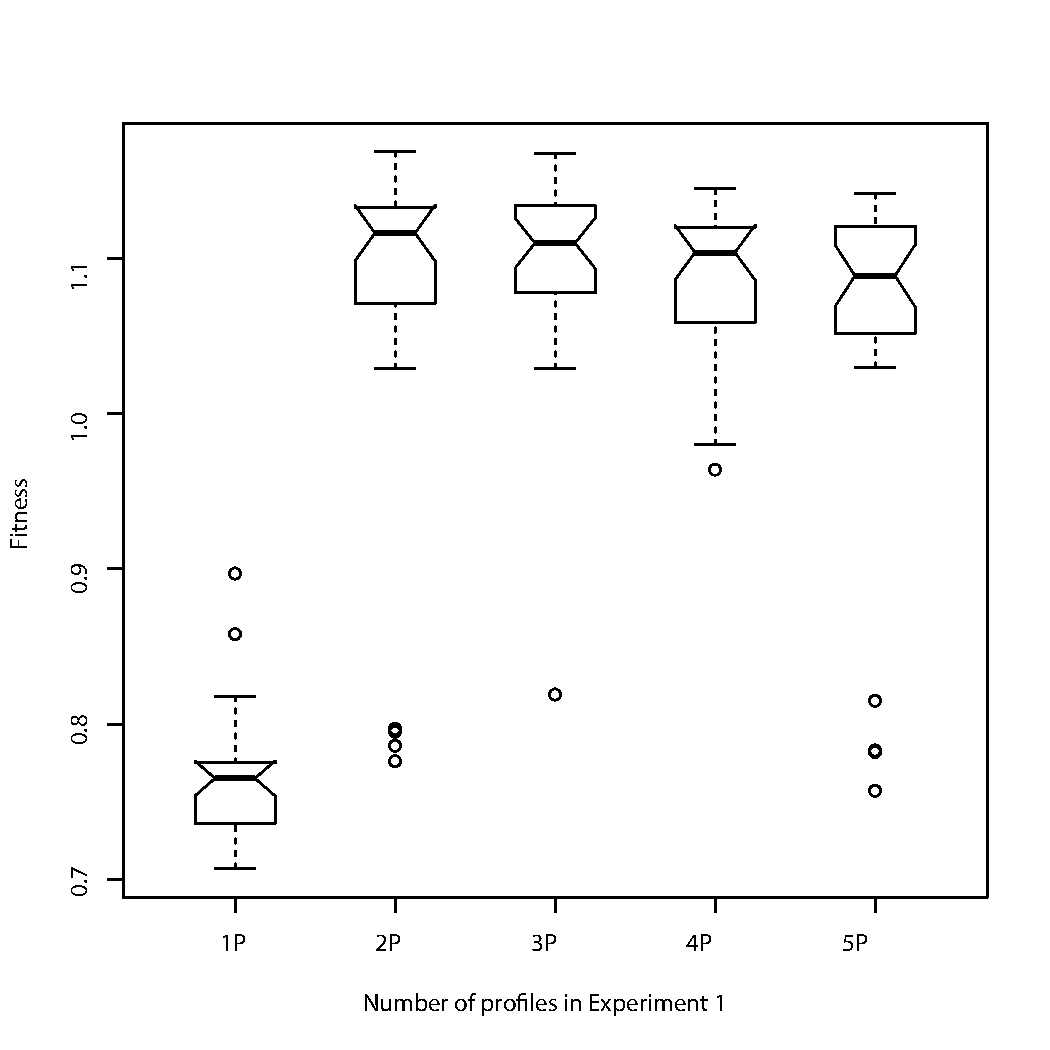
\includegraphics[scale=0.3] {img/exp1_v2.pdf}
   \label{fig:subfig1}
 }
\subfigure[``Revenge'' Setting]{
   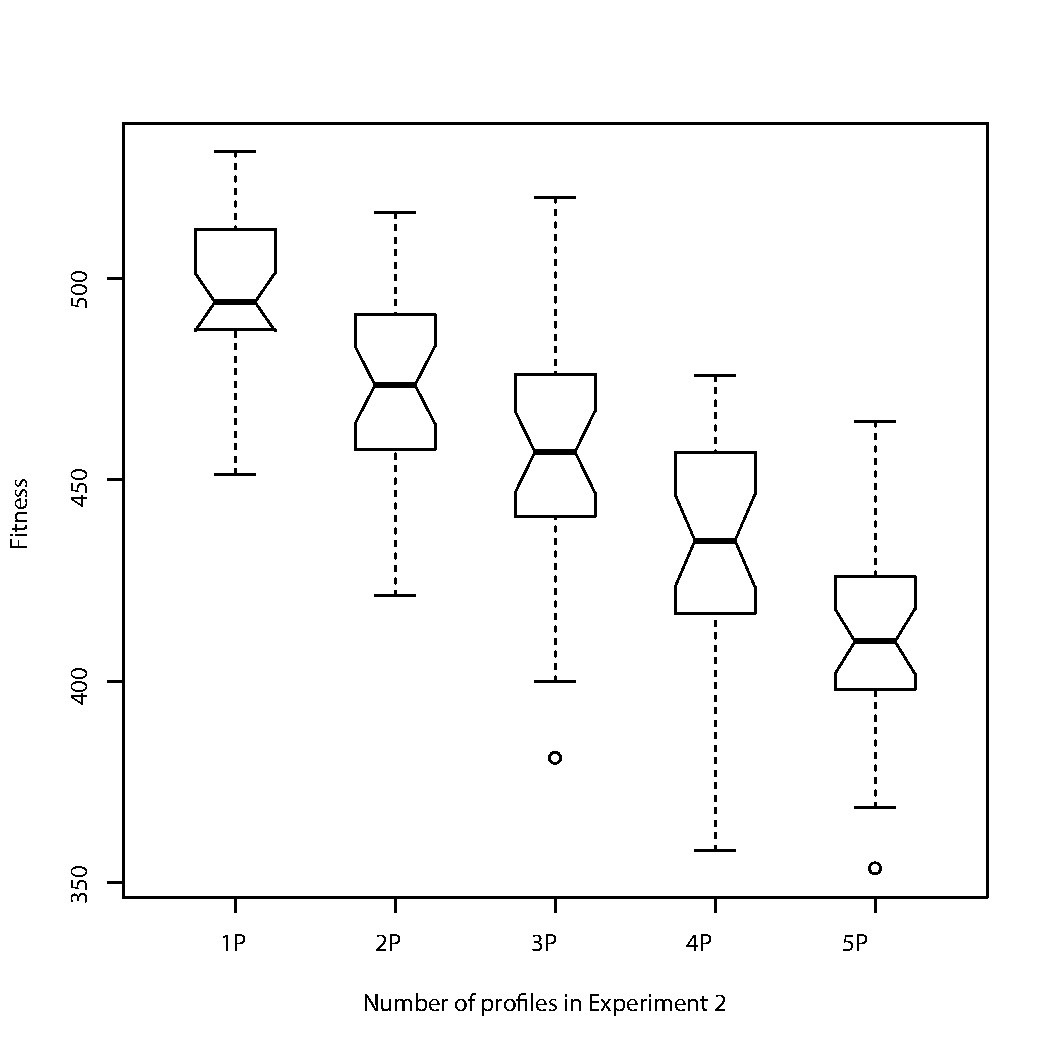
\includegraphics[scale=0.3] {img/exp2_v2.pdf}
   \label{fig:subfig2}
 }
\caption{Average fitness of the 30 best individuals of the GA for each configuration.}

\label{fig:graph}
\end{figure}

Two different literary settings are going to be tested.  The first literary setting, ``territorial war'', aggregates different sample archetypes where many factors must be taken into account.  It tries to find the number of profiles and values that generate at the end of the run an equal distribution of the archetypes \textit{downtrodden} (an agent that has been attacked at least two times and has defended the position), \textit{warrior} (if it has satisfactory attacked at least five times), \textit{helpless} (if it has been defeated 10 times) and \textit{bad warrior} (if it has unsatisfactory attacked at least 10 times). The second literary setting is called ``revenge'' and its goal is to model an individual complex memory
based behavior between two characters:
%This scene is performed to make more complex memory based behavior emerging between two characters:
it tries to find the number of profiles and values which are optimal to make \textit{revenge} archetype emerge in as many agents as possible.  An\textit{avenger} is an agent ({\em a}) that has been attacked by other agent ({\em b}) and, after that, it has satisfactory attacked the agent {\em b}, in \textit{revenge}. For this setting, every agent whose log matches the archetype adds one point to the fitness. %Therefore, the goal is to recreate an environment where several ``avenger'' agents exist.
%\subsection{Definition of  the genetic algorithm}
%To model the ``territorial war'' setting we have defined the fitness function as follows: if the exact percentage of agents are tagged with one archetype defined, 1 point is added to the fitness. The maximum is therefore, 5 points. However, all the fitnesses use a normal distribution over the percentage of appearance. For example, with the archetype ``survival population'', the maximum value (1) is obtained when the 60\% percent of the population is alive, and the normal distribution begins in the 30\% and ends in the 90\%. For the rest of the archetypes, 1 point is reached if the 22'5\% of the population is tagged with each one of the archetypes, and each normal distribution begins in the 8\% and ends in the 30\%.


%Thanks to the agents' logs, we can know every event
%(internal and external)
%of their lives, and evaluate their
%interest or
%adequacy to a specific literary setting. In this work, we have implemented a method based on regular expressions with backreferences.
%The proposed technique puts annotations in every agent whose log matches a complex regular expression able to find emerging high level behaviours, not implemented in the life-cycle.

%In this proposal,
%The parameters used to define an agent, mentioned in Section~\ref{sec:methodology}, are mapped into a chromosome, and a Genetic Algorithm is used to evolve the solution.
%The fitness function is expressed in terms of:

%\begin{itemize}
%\item \textbf{Regular expressions applied to the log of each agent in the environment:} An agent is tagged when a regular expression matches its log.
%\item \textbf{A numeric function over the number of tagged agents for each archetype:} the fitness of the solution is incremented with the returning value.
%\end{itemize}
%


%In this case,
% we do not exactly know how many roles are necessary to create a world of ``warrior'' or ``vindictive''
%  rats, so different number of profiles (from one to five) will be considered.



%If only one profile is used
%in a run, all the agents are created with the same parameters, evolved
%by the Genetic Algorithm. If more profiles are used, they are assigned
%to the agents in order of appearance in a loop. Our assumption is that
%some archetypes could emerge using one profile and other will need
%more (those that require two clearly differentiated roles). It is
%important to remark that the number of alleles of the chromosome are
%multiplied by the number of profiles, so the convergence of the
%solution will be be affected by the number of profiles used. 




%\section{Set up and results}

%For the experiments performed in this work, we have used the parameters shown in Table~\ref{fig:ga_parameters}. These values have been chosen empirically after several test runs.
%
%\begin{table}[htb]
%\begin{center}
%\caption{Parametrization of the Genetic Algorithm}
%\label{fig:ga_parameters}
%\begin{tabular}{cc}%{p{3cm}p{7cm}}
%\hline\noalign{\smallskip}
%\noalign{\smallskip}
%Parameter & Value \\
%\hline
%\noalign{\smallskip}
%Codification & 12 alleles per profile\\
%Fitness function & Average of 10 executions.\\
%Natural selector & Original Rate: 0.9 \\
%Crossover operator & Rate: 35\% \\
%Mutation operator & Desired Rate: 12 \\
%Stop condition & 100 executions\\ % �A qu� se refiere? Esto confund�a
%                                % tambi�n al revisor - JJ PPSN 
%Generations & 30\\
%Population size & 30 \\
%\hline
%\end{tabular}
%
%\end{center}
%\end{table}


%\begin{table}
%\begin{center}
%\caption{Average best fitness for 30 executions of each configuration using 1 to 5 profiles.}
%\label{fig:exp1_30ex}

%\begin{tabular}{lllll}
%\hline\noalign{\smallskip}
%\parbox[t]{1.5cm}{Profiles}
%& \parbox[t]{2cm}{Setting 1}
%& \parbox[t]{2cm}{Setting 2} \\
%\noalign{\smallskip}
%\hline
%\noalign{\smallskip}
%1 & 0,765 $\pm$ 0,037 & 495,513 $\pm$ 20,091 \\
%2 & 1,063 $\pm$ 0,115 & 471,206 $\pm$ 24,550 \\
%3 & 1,093 $\pm$ 0,063 & 455,42 $\pm$ 28,240 \\
%4 & 1,084 $\pm$ 0,048 & 431,926 $\pm$ 31,682 \\
%5 & 1,045 $\pm$ 0,110 & 411,24 $\pm$ 25,023 \\
%\hline
%\end{tabular}
%\end{center}
%\end{table}


The experiments performed in this work uses 12 alleles per profile, a fitness function as the average of ten executions, a natural selector with rate 0.9, a crossover operator with a rate of 35\%, a mutation probability of 1/12, 100 generations and population size of 30 individuals. These values have been chosen empirically after several test runs. To ensure the representativeness of the results, we have executed 30 times each experiment with different number of profiles, from 1 (P1) to 5 (P5). Boxplots of the best fitness obtained are shown in Figures \ref{fig:subfig1} and \ref{fig:subfig2}. In the setting ``Territorial war'', we have performed a Kruskal-Wallis test for the
best individuals fitness, obtaining differences among all the number
of profiles (p-value $<<$ 0.05). It is clear that
using one profile is not enough to emerge the desired
archetype. However, the pairwise comparison using Wilcoxon does not
find significant differences  between the results that use more than
two profiles. In the setting ``revenge'', there are significant differences among all
configurations (p-value $<<$ 0.05) except between P2 and P3
(p-value=0.3). Therefore, we can conclude that in this kind of global
archetype only a profile must be used for obtaining the best
results.








%This can be explained because an agent could share more
%than one archetype at the same time.  A promising number of profiles
%could be 4, because their only lower outlier is not as distributed as
%the others.  

%\begin{table}
%\begin{center}
%\caption{Results for 30 executions of each configuration using 1 to 5 profiles in the experiment 1}
%\label{fig:exp1_30ex}
%
%\begin{tabular}{lllll}
%\hline\noalign{\smallskip}
%\parbox[t]{1.5cm}{Number of\\ profiles}
%& \parbox[t]{2cm}{Best fitness\\ (average) *}
%& \parbox[t]{2cm}{Average\\ fitness **} \\
%\noalign{\smallskip}
%\hline
%\noalign{\smallskip}
%1 & 0,765 $\pm$ 0,037 & 0,761 $\pm$ 0,038 \\
%2 & 1,063 $\pm$ 0,115 & 1,059 $\pm$ 0,114 \\
%3 & 1,093 $\pm$ 0,063 & 1,091 $\pm$ 0,062 \\
%4 & 1,084 $\pm$ 0,048 & 1,082 $\pm$ 0,048 \\
%5 & 1,045 $\pm$ 0,110 & 1,041 $\pm$ 0,108 \\
%\hline
%\end{tabular}
%\\
%\** Average of the best fitness at the end of each execution\\
%% Es decir, coges el mejor fitness de cada ejecucion (tendras 30 por cada
%% numero de perfiles) y sacas la media
%\*** Average population fitness  at the end of each execution \\
%\end{center}
%\end{table}




%The results of the second experiment are shown in
%Table~\ref{fig:exp2_30ex}.
%It shows the average of the best fitness
%and the average population fitness at the end of 30 executions for
%each configuration.

%Table~\ref{fig:exp2_30ex}.
%shows the average of the best fitness and the average population fitness
%%at the end of 30 executions for each configuration: number of profiles from 1 (P1) to 5 (P5) 
%in the experiment 1 (``Revenge'').
%Boxplots of the best fitness obtained are shown
%in Figure \ref{fig:subfig2}.


%This makes sense, because we are looking for one type of
%local archetypes ({\em avenger}), so adding extra profiles leads to
%different behaviours of the agents. 


%\begin{table}
%\begin{center}
%\caption{Results for 30 executions of each configuration using 1 to 5 profiles in the experiment 2}
%\label{fig:exp2_30ex}
%\begin{tabular}{lllll}
%\hline\noalign{\smallskip}
%\parbox[t]{1.5cm}{Number of\\ profiles}
%& \parbox[t]{2cm}{Best fitness\\(average) *}
%& \parbox[t]{2cm}{Average\\fitness **} \\
%\noalign{\smallskip}
%\hline
%\noalign{\smallskip}
%1 & 495,513 $\pm$ 20,091 & 493,908 $\pm$ 19,884 \\
%2 & 471,206 $\pm$ 24,550 & 469,361 $\pm$ 24,015 \\
%3 & 455,42 $\pm$ 28,240 & 452,787 $\pm$ 29,438 \\
%4 & 431,926 $\pm$ 31,682 & 428,206 $\pm$ 31,238 \\
%5 & 411,24 $\pm$ 25,023 & 408,387 $\pm$ 23,829 \\
%\hline
%\end{tabular}
%\\
%\** Average of the best fitness at the end of each execution\\
%\*** Average population fitness  at the end of each execution \\
%
%\end{center}
%\end{table}




\section{Conclusions}
\label{sec:conclusion}



This work presents a general methodology to design emergent literary stories in massive virtual worlds. The described steps include the modeling of the agents and literary setting. Then a Genetic Algorithm is used to optimize the parameters of the agent's profiles (sets of parameters assigned to the agents) using
as fitness a function that models the literary setting by using the concept of {\em archetype}.  The execution of the MADE Environment
using these profiles as input would produce a background (or set of characters' lives)
where the archetypes have emerged and have automatically created massive backstories coherent
with the settings of the artwork. Results show that the optimal number of profiles depends on the number of desired archetypes and their nature.

% In future works, more complex agents could be used, with more complex archetypes and taking into account human opinions to establish the interestingness of a generated plot.
%For example, we plan to model more human behaviors such as love or envy, to generate interesting plots such as wars, weddings, or family crimes. Different fitness functions will be used, for example, taking into account human opinions to establish the interestingness of a generated plot. Also, this system will be tested into an existent and well-known game, such as Skyrim\texttrademark, whose AI engine is publicly available for players and researchers.

% -----------------------------------------------------------------------------
% SEC ACKNOWLEGGEMENTS
% \section{Acknowledgments}



%\section{Acknowledgments}
%This work has been supported in part by FPU research grant AP2009-2942 and TIN2011-28627-C04-02. 
\bibliographystyle{abbrv}
\bibliography{made}  % sigproc.bib is the name of the Bibliography in this case

\end{document}
